\setcounter{section}{32}
\section{Постановка и решение задачи 2SAT (применение алгоритма выделения компонент сильной связности).}
Пусть дана 2-КНФ, формула вида ($\overline{p} \vee q$) $\wedge (p \vee y) \wedge (y \vee \overline{z})$. Будем считать, что дизъюнктов вида $(p \wedge \overline{p}), (p \wedge p)$ нет.
\\ Вопрос: выполнима ли эта формула?
\\
Поступим следующим образом:
\begin{itemize}
    \item [1] Для каждой переменной, входящей в КНФ, запишем саму переменную и ее отрицание
    \item [2] Для каждой скобки вида ($x \vee y$) проведем ориентированное ребро между $\overline{x}$ и y,  $\overline{y}$ и x. В логическом смысле каждая такая скобка будет эквиваленнтна $(\overline{x} \rightarrow$  y) $\wedge (\overline{y} \rightarrow x)$.
\end{itemize}
 Утверждается, что формула выполнима тогда и только тогда, когда $\forall p$, p и ее отрицание не лежат в одной компоненте сильной связности. Почему это так? 
 \begin{itemize}
     \item [$\rightarrow$] Пусть они лежат в одной компоненте сильной связности. Тогда какое значение может принимать p? Пусть единица. Тогда по построению все элементы КСС должны быть равны 1, тогда и $\overline{p} = 1$.  Противоречие. Аналогично р не может принимать значение 0.
     \item [$\leftarrow$] Пусть выполнено условие. Покажем, как построить выполняющий набор для формулы. Вспомним алгоритм Косарайю. Он выделяет КСС в каком-то порядке. Пусть С(v) - номер КСС вершины v в этом порядке. \\ Набор:
     \begin{itemize}
         \item p = 1 $\Longleftrightarrow C(p) > C(\overline{p})$
         \item p = 0 $\Longleftrightarrow C(p) < C(\overline{p})$
     \end{itemize}
     Пусть этот набор не выполним, тогда существует ложный дизъюнкт ($x \vee y$) = 0, а значит,  x = 0, y = 0  $\Longleftrightarrow C(x) < C(\overline{x}),C(y) < C(\overline{y}) $. Если у нас есть такой дизъюнкт, то в графе есть ребра \\ $\overline{x} \rightarrow y \\ \overline{y} \rightarrow x $
     \begin{center}
         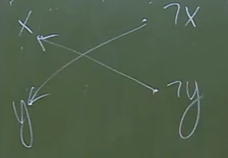
\includegraphics[width=7cm]{images/33_alg16.PNG}
     \end{center}
     $tout[\overline{y}$] $\geq  tout[x]$, а значит $C(\overline{y}) \leq C(x) < C(\overline{x}) \leq C(y) $ - противоречие
 \end{itemize}
 \textbf{Асимптотика} \\
 O(n + m).
 \\
 1. Строим граф с 2n вершинами и 2m ребрами
\\
2. Запускаем алгоритм Косарайю\\
3. Узнаем номера КСС для всех пар (переменная, ее отрицание), проверяем, что они различны\\
4. Строим набор по праввилу, описанному в доказательстве выше